\documentclass{beamer}
\usepackage{graphicx}
\usepackage{listings}
\usetheme{Madrid}

\title{基于UNet的量子关联成像端到端重建系统}
\author{Ivan Tang}
\date{2025年5月}

\begin{document}

% 封面
\frame{\titlepage}

% 项目简介
\begin{frame}{项目简介}
\begin{itemize}
    \item 本项目实现了基于UNet的量子关联成像(Quantum Correlated Imaging)端到端重建系统。
    \item 支持多帧signal/idler图像堆叠为多通道输入,适配UNet结构。
    \item 灵活损失函数组合(SSIM、MSE、感知损失等),支持多种损失加权。
    \item 自动化实验记录与超参数搜索,便于对比和复现。
\end{itemize}
\end{frame}

% 数据结构
\begin{frame}{数据结构与预处理}
\textbf{每个样本目录结构:}
\begin{lstlisting}
object_dir/
  signal/   % 多帧signal图片
  idler/    % 多帧idler图片
  target.JPG
\end{lstlisting}
\vspace{0.5em}
\textbf{多帧堆叠与预叠加:}
\begin{itemize}
    \item 先各自取前max\_signal/max\_idler张signal/idler图片
    \item 每stack\_num张图片做均值叠加,合成为1通道
    \item 最终输入通道数为$(\text{max\_signal}//\text{stack\_num}) + (\text{max\_idler}//\text{stack\_num})$
\end{itemize}
\end{frame}

% 数据流图
\begin{frame}{数据流与输入示意}
\begin{columns}
\column{0.5\textwidth}

\includegraphics[width=0.95\linewidth]{results/target_0.png}
\centerline{\small target样例}
\column{0.5\textwidth}

\includegraphics[width=0.95\linewidth]{results/pred_0.png}
\centerline{\small pred样例}
\end{columns}
\vspace{0.5em}
\textbf{输入张量结构:}
\begin{itemize}
    \item $X$: [C, H, W],C为堆叠后的通道数
    \item target: [1, H, W]
\end{itemize}
\end{frame}

% 模型架构
\begin{frame}{模型架构——UNet}
\begin{itemize}
    \item 采用标准UNet结构,支持自定义in\_channels,适配多通道输入
    \item 编码器-解码器对称结构,跨层跳连
    \item 输出为单通道重建图像
\end{itemize}
\begin{center}
\includegraphics[width=0.8\linewidth]{https://raw.githubusercontent.com/milesial/Pytorch-UNet/master/img/unet-architecture.png}
\end{center}
\textit{(如需自定义结构,可直接修改model.py)}
\end{frame}

% 损失函数与训练流程
\begin{frame}{损失函数与训练流程}
\begin{itemize}
    \item 支持SSIM、MSE、感知损失(VGG16)等多种损失加权组合
    \item 损失函数示例:
\end{itemize}
\begin{lstlisting}[language=Python]
def loss_fn(output, target):
    return w_ssim * (1 - ssim(output, target)) \
         + w_mse * MSELoss(output, target) \
         + w_perc * perceptual_loss(output, target)
\end{lstlisting}
\begin{itemize}
    \item 自动保存最优模型、loss曲线、PSNR曲线等
    \item 每次实验自动归档,便于对比
\end{itemize}
\end{frame}

% 超参数搜索与实验记录
\begin{frame}{超参数搜索与实验记录}
\begin{itemize}
    \item 支持Optuna自动化超参数搜索,参数包括stack\_num、learning\_rate、max\_signal、损失权重等
    \item 每次搜索自动记录所有trial结果与最优参数
    \item 每次训练自动生成唯一实验名,所有结果归档于results/exp\_xxx/
\end{itemize}
\begin{lstlisting}[language=Python]
study = optuna.create_study(direction='minimize')
study.optimize(objective, n_trials=20)
\end{lstlisting}
\end{frame}

% 可视化与样例输出
\begin{frame}{实验可视化与样例输出}
\begin{columns}
\column{0.5\textwidth}
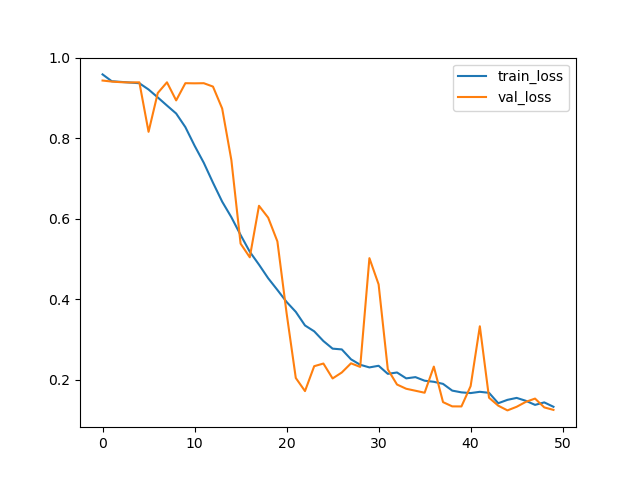
\includegraphics[width=0.95\linewidth]{results/losses.png}
\centerline{\small loss曲线}
\column{0.5\textwidth}
% 如未生成psnrs.png,可用注释占位
%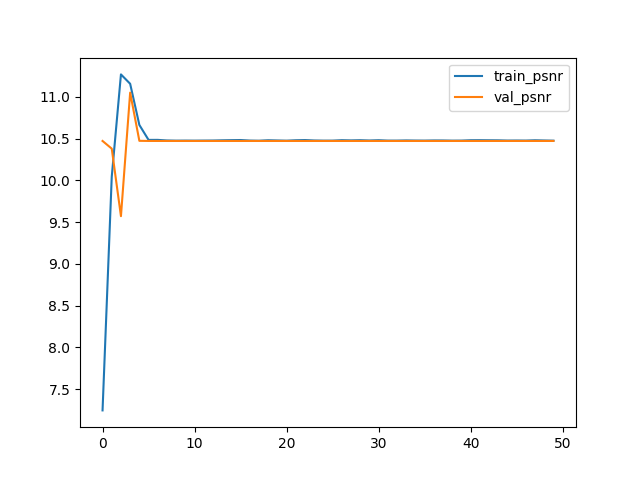
\includegraphics[width=0.95\linewidth]{results/exp_xxx/psnrs.png}
\centerline{\small PSNR曲线(示意)}
\end{columns}
\vspace{0.5em}
\begin{itemize}
    \item 预测结果与目标图像对比见上一页
    \item 更多样例可在results/目录下查看
\end{itemize}
\end{frame}

% 主要参数与调参建议
\begin{frame}{主要参数与调参建议}
\begin{itemize}
    \item stack\_num、max\_signal、损失权重等建议先手动粗调,再用Optuna等自动化工具细调
    \item PSNR/SSIM 只用于评估,不建议作为loss
    \item 代码高度模块化,便于自定义感知损失、模型结构、数据处理等
\end{itemize}
\end{frame}

% PSNR 指标说明
\begin{frame}{PSNR 指标说明}
    \textbf{PSNR(峰值信噪比, Peak Signal-to-Noise Ratio)} 是衡量图像重建质量的常用指标,单位为 dB(分贝)。
    \begin{itemize}
        \item \textbf{定义:} $\mathrm{PSNR} = 10 \log_{10}(\mathrm{MAX}^2 / \mathrm{MSE})$
        \item \textbf{MAX} 为像素最大值(如1.0或255),MSE为均方误差
        \item \textbf{范围:} 理论上 $[0, +\infty)$,实际常见 $10\sim40$ dB
        \item \textbf{常见区间:}
        \begin{itemize}
            \item $<20$ dB:肉眼可见明显失真
            \item $20\sim30$ dB:有失真但可接受
            \item $30\sim40$ dB:高质量重建
            \item $>40$ dB:几乎无失真
        \end{itemize}
        \item \textbf{PSNR 越高,重建效果越好}
        \item 本项目所有PSNR均基于归一化到$[0,1]$的灰度图像
    \end{itemize}
\end{frame}
% --- END ---

% 结语
\begin{frame}{结语}
\begin{itemize}
    \item 项目已实现端到端量子关联成像重建、自动实验归档与超参数搜索
    \item 欢迎交流与贡献,详见README.md
\end{itemize}
\end{frame}

\end{document}
